\chapter[Leçon 36: En Noruff an der Zeitung -- Erënnerung a Sproochelementer]{Leçon 36: En Noruff an der Zeitung -- Erënnerung, Gefiller a Sproochelementer}

Dës Lektioun baséiert op der gemeinsamer Analys vun engem authenteschen Text aus der Lëtzebuerger Zeitung: engem \textbf{Noruff} (Annonce d'anniversaire / in memoriam) fir de Raymond Even. Mir kucken eis d'Sprooch vun der Erënnerung an der Trauer un, léiere wichteg Ënnerscheeder tëscht Verbe wéi \textbf{vermëssen}, \textbf{feelen} a \textbf{fillen}, analyséieren Ausdréck wéi \textbf{wéi doen} an \textbf{ëm Rot froen}, klären de grammatikaleschen Ënnerscheed tëscht \textbf{an Trauer} a \textbf{am Trauer}, a behandele souwuel de Konditiounssaz (\textit{géif}) wéi och d'Nominaliséierung vun däitleche Verben (\textit{dat Zesummesinn}, \textit{dat Plangen}, \textit{dat Sträiden}, \textit{dat Laachen}).

\textit{Cette leçon est consacrée à l'analyse détaillée d'un texte authentique extrait de la presse luxembourgeoise : un avis commémoratif / hommage posthume (\textbf{en Noruff}) en mémoire de Raymond Even. Nous étudions le vocabulaire du souvenir et du deuil, la distinction entre \textbf{an Trauer} et \textbf{am Trauer}, les nuances essentielles entre \textbf{vermëssen} (regretter l'absence de), \textbf{feelen} (manquer / faire défaut) et \textbf{fillen} (ressentir), l'expression de la douleur (\textbf{wéi doen}), la demande de conseil (\textbf{ëm Rot froen}), ainsi que l'emploi du conditionnel (\textit{géif}) et la nominalisation des verbes (\textit{dat Zesummesinn}, \textit{dat Plangen}, etc.).}

\textit{This lesson is dedicated to the detailed analysis of an authentic text from the Luxembourg press: a memorial anniversary announcement / obituary notice (\textbf{en Noruff}) in memory of Raymond Even. We explore the vocabulary of memory and mourning, the grammatical distinction between \textbf{an Trauer} and \textbf{am Trauer}, the crucial distinctions between \textbf{vermëssen} (to emotionally miss), \textbf{feelen} (to be missing/lacking), and \textbf{fillen} (to feel), physical and emotional pain expressions (\textbf{wéi doen}), asking for guidance (\textbf{ëm Rot froen}), conditional phrasing (\textit{géif}), and nominalized verbs (\textit{dat Zesummesinn}, \textit{dat Plangen}, etc.).}

\vspace{1.5em}

\section[Den Text: En Noruff an der Zeitung / The Article]{Den Text: En Noruff fir de Raymond \\/ Le texte : Un hommage commémoratif dans le journal \\/ The Text: A Memorial Notice in the Newspaper}

\subsection*{De ganzen Text / Texte intégral / Full Uncut Text}

\begin{center}
\fbox{
\parbox{0.92\textwidth}{
\vspace{0.4em}
\centering
\textbf{\Large Raymond} \\[0.3em]
\textbf{20. Februar 1961 -- 1. Oktober 2025} \\[1em]
\raggedright
Et ass elo ee Joer hier, dass du eis fir ëmmer verlooss hues. \\[0.4em]
Mee all Dag ginn ech un dech erënnert, an et deet nach ëmmer esou wéi. \\[0.4em]
Et ginn esou vill Momenter a Situatiounen, wou ech dech gär ëm Rot froe géif, \\[0.4em]
wou ech gär mat dir schwätze géif, oder einfach deng Presenz vermëssen, \\[0.4em]
a géif soen: domat ech net eleng. \\[0.4em]
Ech vermëssen dech all Dag méi, an et ass esou schwéier, dech net méi bei eis ze hunn. \\[0.4em]
Deng Presenz, einfach ze wëssen, dass du do bass, feelt eis all Dag méi. \\[0.4em]
Awer du bass weiderhin all Dag bei eis an eisen Häerzer. \\[0.4em]
Mir denken un déi vill schéin Momenter zréck, déi mir zesumme verbruecht hunn: \\[0.4em]
Dat Zesummesinn, dat Plangen, dat Sträiden an dat Laachen, \\[0.4em]
an all déi kleng a grouss Momenter, déi eis zesumme gepräägt hunn. \\[0.4em]
46 Joer zesummen. Dat vergiess een ni. \\[0.4em]
46 Joer voller schéiner Momenter, awer och duerch gutt a schwéier Zäiten, déi mir zesumme gemeeschtert hunn. \\[0.4em]
Du bleifs fir ëmmer an eisen Häerzer. \\[0.4em]
Mir wäerten dech ni vergiessen. \\[0.8em]
\raggedleft
\textbf{Deng Fra Thérèse a Famill an Trauer.} \\[0.3em]
\textit{Bridel, den 3. Oktober 2026}
\vspace{0.4em}
}}
\end{center}

\vspace{1.2em}

\subsection*{Saz fir Saz Analys / Analyse phrase par phrase / Sentence-by-Sentence Breakdown}

\begin{enumerate}
    \item \textbf{Et ass elo ee Joer hier, dass du eis fir ëmmer verlooss hues.}
    \begin{itemize}
        \item \textit{Français :} Cela fait maintenant un an que tu nous as quittés pour toujours.
        \item \textit{English:} It has now been a year since you left us forever.
        \item \textit{Note (FR) :} \textbf{ee Joer hier} = il y a un an (l'adverbe \textit{hier} exprime l'antériorité temporelle : « il y a » ; à ne pas confondre avec le pronom possessif \textit{hir} = sa/leur). Le verbe \textbf{verloossen} (participe passé : \textit{verlooss}) signifie « quitter » ou « abandonner ».
        \item \textit{Note (EN) :} \textbf{ee Joer hier} = a year ago (the temporal adverb \textit{hier} marks time elapsed: "ago"; do not confuse with the possessive pronoun \textit{hir} = her/their). The verb \textbf{verloossen} (past participle: \textit{verlooss}) means "to leave" or "to abandon".
    \end{itemize}

    \vspace{0.6em}

    \item \textbf{Mee all Dag ginn ech un dech erënnert, an et deet nach ëmmer esou wéi.}
    \begin{itemize}
        \item \textit{Français :} Mais chaque jour je me souviens de toi (je suis rappelé(e) à toi), et cela fait toujours aussi mal.
        \item \textit{English:} But every day I am reminded of you, and it still hurts so much.
        \item \textit{Note (FR) :} \textbf{all Dag} = chaque jour / tous les jours (par opposition à \textbf{de ganzen Dag} = toute la journée). La forme passive \textbf{ginn erënnert un} (+ Akkusativ) signifie « être rappelé(e) au souvenir de ». L'expression \textbf{et deet wéi} signifie « ça fait mal » (du verbe \textit{wéidoen}).
        \item \textit{Note (EN) :} \textbf{all Dag} = every day / each day (distinct from \textbf{de ganzen Dag} = the whole day). The passive construction \textbf{ginn erënnert un} (+ accusative) means "to be reminded of". The idiomatic expression \textbf{et deet wéi} means "it hurts" (from the compound verb \textit{wéidoen}).
    \end{itemize}

    \vspace{0.6em}

    \item \textbf{Et ginn esou vill Momenter a Situatiounen, wou ech dech gär ëm Rot froe géif,}
    \begin{itemize}
        \item \textit{Français :} Il y a tellement de moments et de situations où j'aimerais te demander conseil,
        \item \textit{English:} There are so many moments and situations where I would like to ask you for advice,
        \item \textit{Note (FR) :} \textbf{Et ginn} = il y a (employé devant un nom au pluriel, tandis que \textit{et gëtt} s'emploie au singulier). L'expression \textbf{ëm Rot froen} prend obligatoirement la préposition \textbf{ëm}. \textbf{froe géif} est une forme de conditionnel exprimant le souhait et la politesse.
        \item \textit{Note (EN) :} \textbf{Et ginn} = there are (used with plural nouns, whereas \textit{et gëtt} is used for singular). The collocation \textbf{ëm Rot froen} strictly requires the preposition \textbf{ëm}. \textbf{froe géif} is a conditional clause expressing a wish.
    \end{itemize}

    \vspace{0.6em}

    \item \textbf{wou ech gär mat dir schwätze géif, oder einfach deng Presenz vermëssen,}
    \begin{itemize}
        \item \textit{Français :} où j'aimerais parler avec toi, ou simplement où ta présence me manque,
        \item \textit{English:} where I would love to talk with you, or simply miss your presence,
        \item \textit{Note (FR) :} \textbf{deng Presenz} (f.) = ta présence. Le verbe \textbf{vermëssen} exprime le sentiment affectif de manque personnel.
        \item \textit{Note (EN) :} \textbf{deng Presenz} (f.) = your presence. The verb \textbf{vermëssen} conveys the emotional and affective longing for someone.
    \end{itemize}

    \vspace{0.6em}

    \item \textbf{a géif soen: domat ech net eleng.}
    \begin{itemize}
        \item \textit{Français :} et où je dirais : pour que je ne sois pas seule (avec cette peine).
        \item \textit{English:} and would say: so that I am not alone (with this grief).
        \item \textit{Note (FR) :} Remarquez l'ellipse expressive du verbe \textit{sinn} dans cette formule orale authentique : \textit{domat ech net eleng} équivaut à \textit{dass ech domat net eleng sinn}. L'orthographe officielle (LOD) admet \textbf{eleng} ou \textbf{aleng} (avec un seul « l », jamais \textit{alleng}).
        \item \textit{Note (EN) :} Notice the expressive ellipsis of the auxiliary verb \textit{sinn} in this authentic spoken phrasing: \textit{domat ech net eleng} functions as \textit{dass ech domat net eleng sinn} (so that I'm not alone in this sorrow). Official LOD spelling is \textbf{eleng} or \textbf{aleng} (always with a single 'l', never *alleng*).
    \end{itemize}

    \vspace{0.6em}

    \item \textbf{Ech vermëssen dech all Dag méi, an et ass esou schwéier, dech net méi bei eis ze hunn.}
    \begin{itemize}
        \item \textit{Français :} Tu me manques chaque jour davantage, et il est si difficile de ne plus t'avoir auprès de nous.
        \item \textit{English:} I miss you more each day, and it is so hard not having you with us anymore.
        \item \textit{Note (FR) :} La proposition infinitive avec \textit{ze} s'emploie après l'adjectif attribut : \textbf{bei eis ze hunn}.
        \item \textit{Note (EN) :} The infinitive clause with \textit{ze} is triggered following the predicate adjective: \textbf{bei eis ze hunn}.
    \end{itemize}

    \vspace{0.6em}

    \item \textbf{Deng Presenz, einfach ze wëssen, dass du do bass, feelt eis all Dag méi.}
    \begin{itemize}
        \item \textit{Français :} Ta présence, le simple fait de savoir que tu es là, nous manque chaque jour davantage.
        \item \textit{English:} Your presence, simply knowing that you are there, is missing for us more every day.
        \item \textit{Note (FR) :} Ici, le sujet grammatical est \textit{Deng Presenz}, ce qui amène le verbe \textbf{feelen} (manquer / faire défaut : \textit{feelt eis}).
        \item \textit{Note (EN) :} Here, the grammatical subject is \textit{Deng Presenz}, requiring the verb \textbf{feelen} (to be lacking / missing: \textit{feelt eis}).
    \end{itemize}

    \vspace{0.6em}

    \item \textbf{Awer du bass weiderhin all Dag bei eis an eisen Häerzer.}
    \begin{itemize}
        \item \textit{Français :} Mais tu demeures chaque jour auprès de nous dans nos cœurs.
        \item \textit{English:} But you remain with us every day in our hearts.
        \item \textit{Note (FR) :} \textbf{weiderhin} = continuellement, toujours, à l'avenir aussi. Au datif pluriel, \textit{d'Häerzer} donne \textbf{an eisen Häerzer} (rétention du -n devant la consonne 'H').
        \item \textit{Note (EN) :} \textbf{weiderhin} = still, continuously, in the future as well. In the dative plural, \textit{d'Häerzer} becomes \textbf{an eisen Häerzer} (retaining -n before consonant 'H' under Eifeler Regel).
    \end{itemize}

    \vspace{0.6em}

    \item \textbf{Mir denken un déi vill schéin Momenter zréck, déi mir zesumme verbruecht hunn:}
    \begin{itemize}
        \item \textit{Français :} Nous repensons à tous ces beaux moments que nous avons passés ensemble :
        \item \textit{English:} We look back on the many wonderful moments that we spent together:
        \item \textit{Note (FR) :} Le verbe prépositionnel \textbf{zréckdenken un (+ Akkusativ)} signifie « repenser à ». Le verbe irrégulier \textbf{verbréngen} fait son participe passé en \textbf{verbruecht} (\textit{mir hu verbruecht}).
        \item \textit{Note (EN) :} The prepositional verb \textbf{zréckdenken un (+ accusative)} means "to look back on / reflect upon". The irregular verb \textbf{verbréngen} forms its past participle as \textbf{verbruecht} (\textit{mir hu verbruecht}).
    \end{itemize}

    \vspace{0.6em}

    \item \textbf{Dat Zesummesinn, dat Plangen, dat Sträiden an dat Laachen,}
    \begin{itemize}
        \item \textit{Français :} La vie à deux, les projets, les disputes et les éclats de rire,
        \item \textit{English:} Being together, making plans, the arguments, and the laughter,
        \item \textit{Note (FR) :} Quatre infinitifs substantivés neutres avec l'article \textbf{dat} : \textit{zesummesinn} $\rightarrow$ \textit{dat Zesummesinn}, \textit{plangen} $\rightarrow$ \textit{dat Plangen}, \textit{sech sträiden} $\rightarrow$ \textit{dat Sträiden}, \textit{laachen} $\rightarrow$ \textit{dat Laachen}.
        \item \textit{Note (EN) :} Four nominalized neuter infinitives taking the definite article \textbf{dat}: \textit{zesummesinn} $\rightarrow$ \textit{dat Zesummesinn}, \textit{plangen} $\rightarrow$ \textit{dat Plangen}, \textit{sech sträiden} $\rightarrow$ \textit{dat Sträiden}, \textit{laachen} $\rightarrow$ \textit{dat Laachen}.
    \end{itemize}

    \vspace{0.6em}

    \item \textbf{an all déi kleng a grouss Momenter, déi eis zesumme gepräägt hunn.}
    \begin{itemize}
        \item \textit{Français :} et tous ces petits et grands moments qui nous ont façonnés et marqués ensemble.
        \item \textit{English:} and all those small and big moments that shaped and marked us together.
        \item \textit{Note (FR) :} Le verbe \textbf{prägen} (participe passé : \textbf{gepräägt}) signifie « marquer profondément, façonner l'identité de quelqu'un ».
        \item \textit{Note (EN) :} The verb \textbf{prägen} (past participle: \textbf{gepräägt}) means "to stamp, leave a lasting impression on, shape".
    \end{itemize}

    \vspace{0.6em}

    \item \textbf{46 Joer zesummen. Dat vergiess een ni.}
    \begin{itemize}
        \item \textit{Français :} 46 ans ensemble. On n'oublie jamais cela.
        \item \textit{English:} 46 years together. One never forgets that.
        \item \textit{Note (FR) :} \textbf{vergiessen} (3e pers. sing. : \textit{vergiess}) = oublier. Le pronom indéfini \textbf{een} correspond au français « on ».
        \item \textit{Note (EN) :} \textbf{vergiessen} (3rd person sing.: \textit{vergiess}) = to forget. The indefinite pronoun \textbf{een} translates to "one / someone".
    \end{itemize}

    \vspace{0.6em}

    \item \textbf{46 Joer voller schéiner Momenter, awer och duerch gutt a schwéier Zäiten, déi mir zesumme gemeeschtert hunn.}
    \begin{itemize}
        \item \textit{Français :} 46 ans remplis de beaux moments, mais aussi à travers des temps heureux et difficiles, que nous avons surmontés ensemble.
        \item \textit{English:} 46 years full of beautiful moments, but also through good and difficult times, which we mastered together.
        \item \textit{Note (FR) :} \textbf{meeschteren} (participe passé : \textbf{gemeeschtert}) = maîtriser, surmonter, faire face avec succès.
        \item \textit{Note (EN) :} \textbf{meeschteren} (past participle: \textbf{gemeeschtert}) = to master, manage, overcome together.
    \end{itemize}

    \vspace{0.6em}

    \item \textbf{Du bleifs fir ëmmer an eisen Häerzer. Mir wäerten dech ni vergiessen.}
    \begin{itemize}
        \item \textit{Français :} Tu restes pour toujours dans nos cœurs. Nous ne t'oublierons jamais.
        \item \textit{English:} You remain forever in our hearts. We will never forget you.
        \item \textit{Note (FR) :} Le futur est formé avec l'auxiliaire \textbf{wäerten} : \textit{Mir wäerten dech ni vergiessen}.
        \item \textit{Note (EN) :} The future tense is formed using the auxiliary \textbf{wäerten}: \textit{Mir wäerten dech ni vergiessen}.
    \end{itemize}

    \vspace{0.6em}

    \item \textbf{Deng Fra Thérèse a Famill an Trauer.} \\
    \textbf{Bridel, den 3. Oktober 2026.}
    \begin{itemize}
        \item \textit{Français :} Ton épouse Thérèse et la famille en deuil. Bridel, le 3 octobre 2026.
        \item \textit{English:} Your wife Thérèse and the family in mourning. Bridel, 3 October 2026.
        \item \textit{Note (FR) :} \textbf{an Trauer} = en deuil. \textbf{Bridel} est une localité au sud de la commune de Kopstal (canton de Capellen).
        \item \textit{Note (EN) :} \textbf{an Trauer} = in mourning. \textbf{Bridel} is a town in the municipality of Kopstal (canton of Capellen).
    \end{itemize}
\end{enumerate}

\vspace{1.5em}

\section[Vokabelen an Ausdréck / Vocabulary \& Expressions]{Kärvokabelen an Ausdréck aus dem Cours \\/ Vocabulaire essentiel et expressions du cours \\/ Core Vocabulary and Expressions from the Lesson}

\begin{itemize}
    \item \textbf{en Noruff} (m., Pl. \textit{d'Noriffer} / \textit{d'Noruffer}):
    \begin{itemize}
        \item \textit{Bedeitung / Meaning:} Une nécrologie, un hommage commémoratif posthume / obituary, memorial tribute.
        \item \textit{Originn / Etymology:} Composé du préfixe \textit{no-} (après, post-) et de \textit{Ruff} (appel, cri). Équivalent exact de l'allemand \textit{Nachruf}.
        \item \textit{Français :} Nécrologie, éloge funèbre, avis commémoratif.
        \item \textit{English:} Obituary, memorial notice, in memoriam tribute.
        \item \textit{Beispill:} \textit{D'Famill huet e ganz beréierenden Noruff an d'Zeitung gesat.}
        $\rightarrow$ \textit{Français :} La famille a publié une nécrologie très émouvante dans le journal.
        $\rightarrow$ \textit{English:} The family published a very touching obituary notice in the newspaper.
    \end{itemize}

    \vspace{0.6em}

    \item \textbf{sech erënneren un (+ Akkusativ)} / \textbf{erënnert ginn un}:
    \begin{itemize}
        \item \textit{Bedeitung / Meaning:} Se souvenir de / être rappelé(e) à ; to remember / to be reminded of.
        \item \textit{Aussprooch (LOD):} [ɐʀˈənəʀən]
        \item \textit{Grammaire (FR) :} Se construit obligatoirement avec la préposition \textbf{un} (+ Akkusativ) : \textit{Ech erënnere mech un hien} (Je me souviens de lui). Au passif : \textit{Mee all Dag ginn ech un dech erënnert.} (Chaque jour, ton souvenir m'est rappelé).
        \item \textit{Grammar (EN):} Strictly constructed with the preposition \textbf{un} (+ accusative): \textit{Ech erënnere mech un hien} (I remember him). In the passive: \textit{Mee all Dag ginn ech un dech erënnert.} (Every day, I am reminded of you).
    \end{itemize}

    \vspace{0.6em}

    \item \textbf{wéi doen} (onreegelméissegt Verb, pp. \textit{wéigedoen}):
    \begin{itemize}
        \item \textit{Bedeitung / Meaning:} Faire mal, être douloureux / to hurt, to cause pain.
        \item \textit{Grammaire (FR) :} Composé de l'adverbe \textit{wéi} (mal, douloureux) et du verbe \textit{doen} (faire).
        \item \textit{Grammar (EN):} Formed from the adverb \textit{wéi} (painful) and the verb \textit{doen} (to do/make).
        \item \textit{Présent / Present:} \textit{Et deet wéi} (Ça fait mal / It hurts).
        \item \textit{Froen an Ausdréck aus der Praxis / Practical phrases:}
        \begin{itemize}
            \item \textit{Wou deet et wéi?} $\rightarrow$ \textit{FR:} Où avez-vous mal ? / \textit{EN:} Where does it hurt?
            \item \textit{Wou deet et dir wéi?} $\rightarrow$ \textit{FR:} Où as-tu mal ? / \textit{EN:} Where does it hurt you?
            \item \textit{Mäi Kapp deet wéi.} $\rightarrow$ \textit{FR:} J'ai mal à la tête. / \textit{EN:} My head hurts.
            \item \textit{Mäi Réck deet wéi.} $\rightarrow$ \textit{FR:} J'ai mal au dos. / \textit{EN:} My back hurts.
            \item \textit{Meng Hand deet wéi.} $\rightarrow$ \textit{FR:} J'ai mal à la main. / \textit{EN:} My hand hurts.
        \end{itemize}
    \end{itemize}

    \vspace{0.6em}

    \item \textbf{ëm Rot froen} / \textbf{ëm Hëllef froen}:
    \begin{itemize}
        \item \textbf{de Rot} (m., Pl. \textit{d'Réit}) = Le conseil / Advice.
        \item \textit{Français :} Demander conseil / demander de l'aide.
        \item \textit{English:} To ask for advice / to ask for help.
        \item \textit{Prepositioun (FR) :} On utilise obligatoirement la préposition \textbf{ëm} : \textit{Ech géif dech gär ëm Rot froen.}
        \item \textit{Preposition (EN):} The construction strictly takes the preposition \textbf{ëm}: \textit{Ech géif dech gär ëm Rot froen.} (I would like to ask you for advice).
    \end{itemize}

    \vspace{0.6em}

    \item \textbf{vermëssen} vs \textbf{feelen} vs \textbf{fillen} vs \textbf{e Fëllen}:
    \begin{itemize}
        \item \textbf{vermëssen} (hunn vermësst):
        \begin{itemize}
            \item \textit{Français :} Manque \textit{affectif} et émotionnel (regretter l'absence de quelqu'un ou de quelque chose de cher).
            \item \textit{English:} Emotional/affective longing (to miss someone or a beloved memory).
            \item \textit{Beispill 1:} \textit{Ech vermëssen dech all Dag.} $\rightarrow$ \textit{FR:} Tu me manques chaque jour. / \textit{EN:} I miss you every day.
            \item \textit{Beispill 2:} \textit{Ech vermëssen d'Kiche vu menger Mamm.} $\rightarrow$ \textit{FR:} La cuisine de ma mère me manque. / \textit{EN:} I miss my mother's cooking.
        \end{itemize}

        \item \textbf{feelen} (huet gefeelt):
        \begin{itemize}
            \item \textit{Français :} Manque \textit{objectif}, absence physique, déficit ou pénurie.
            \item \textit{English:} Objective absence, lack, shortage, or being missing.
            \item \textit{Beispill 1:} \textit{Haut feelen dräi Schüler am Cours.} $\rightarrow$ \textit{FR:} Aujourd'hui, trois élèves manquent au cours. / \textit{EN:} Today, three students are absent from class.
            \item \textit{Beispill 2:} \textit{Et feelt eis u Suen.} $\rightarrow$ \textit{FR:} Nous manquons d'argent. / \textit{EN:} We lack money.
            \item \textit{Beispill 3:} \textit{Deng Presenz feelt eis.} $\rightarrow$ \textit{FR:} Ta présence nous fait défaut. / \textit{EN:} Your presence is missing to us.
        \end{itemize}

        \item \textbf{sech fillen} (huet sech gefillt):
        \begin{itemize}
            \item \textit{Français :} Se sentir (sensation physique ou morale).
            \item \textit{English:} To feel (physical or emotional state).
            \item \textit{Beispill:} \textit{Ech fille mech haut ganz fit.} $\rightarrow$ \textit{FR:} Je me sens très en forme aujourd'hui. / \textit{EN:} I feel very fit today.
        \end{itemize}

        \item \textbf{e Fëllen} (n., Pl. \textit{d'Fëllen}):
        \begin{itemize}
            \item \textit{Français :} Le poulain (le petit du cheval). Genre neutre, voyelle brève \textit{ë}.
            \item \textit{English:} The foal / young horse. Neuter noun, short vowel \textit{ë}.
            \item \textit{Beispill:} \textit{D'Mier steet mat hirem klenge Fëllen op der Wiss.} $\rightarrow$ \textit{FR:} La jument se tient avec son petit poulain dans le pré. / \textit{EN:} The mare is standing with her little foal in the meadow.
        \end{itemize}
    \end{itemize}

    \vspace{0.6em}

    \item \textbf{eleng} / \textbf{aleng}:
    \begin{itemize}
        \item \textit{LOD-Norm :} Les deux formes officielles sont \textbf{eleng} et \textbf{aleng} (toutes deux écrites avec un seul « l », jamais *\textit{alleng}*).
        \item \textit{Français :} Seul(e), tout(e) seul(e), isolé(e).
        \item \textit{English:} Alone, by oneself, on one's own.
        \item \textit{Beispill 1 :} \textit{Domat bass du net eleng.} $\rightarrow$ \textit{FR:} Tu n'es pas seul(e) avec cela. / \textit{EN:} You are not alone with that.
        \item \textit{Beispill 2 :} \textit{Hie wunnt aleng an engem Appartement.} $\rightarrow$ \textit{FR:} Il vit seul dans un appartement. / \textit{EN:} He lives alone in an apartment.
    \end{itemize}

    \vspace{0.6em}

    \item \textbf{meeschteren} (transitiivt Verb, gemeeschtert hunn):
    \begin{itemize}
        \item \textit{Français :} Maîtriser, surmonter, faire face à, gérer avec succès.
        \item \textit{English:} To master, to overcome, to cope with, to manage successfully.
        \item \textit{Beispill :} \textit{Zesummen hu mir all Schwieregkeete gemeeschtert.}
        $\rightarrow$ \textit{Français :} Ensemble, nous avons surmonté toutes les difficultés.
        $\rightarrow$ \textit{English:} Together, we managed and overcame all difficulties.
    \end{itemize}

    \vspace{0.6em}

    \item \textbf{d'Trauer} (f.) vs \textbf{den Trauer} (m.) / \textbf{an Trauer} vs \textbf{am Trauer}:
    \begin{itemize}
        \item \textbf{D'Fro / La question linguistique :} Dit-on \textit{d'Famill an Trauer} ou \textit{d'Famill am Trauer} ? Est-ce \textit{d'Trauer} (féminin) ou \textit{den Trauer} (masculin) ?
        \item \textit{Recherche vum Prof. Dr. Peter Gilles (Uni Lëtzebuerg / Infolux / RTL.lu) :}
        \begin{itemize}
            \item \textbf{d'Trauer} (f.) désigne avant tout le \textit{sentiment intérieur}, l'émotion de peine et de tristesse. C'est la forme dominante dans l'usage contemporain et dans les avis de décès : \textbf{D'Famill an Trauer} (la famille en deuil) ou \textit{an déiwer Trauer sinn} (être dans un profond deuil).
            \item \textbf{den Trauer} (m.) se réfère au \textit{deuil concret}, à la période officielle ou extérieure de deuil, ou aux vêtements noirs de deuil. On dit ainsi : \textbf{am Trauer sinn} (porter le deuil, être en période de deuil). Le mot \textit{am} est la contraction de \textit{an dem} (datif masculin).
            \item \textit{Historeschen Hannergrond :} Dans l'ancien \textit{Luxemburger Wörterbuch} (LWB), le mot était principalement répertorié comme masculin (\textit{den Trauer}), avec la mention que le féminin apparaissait nouvellement. Une hypothèse linguistique suggère que \textit{den Trauer} dérive de l'ellipse d'un composé comme *\textit{den Trauerzoustand}* (l'état de deuil) ou *\textit{den Trauerdag}*, analogue à *\textit{de Kanddaf}* (masculin issu de *\textit{de Kanddafdag}*).
        \end{itemize}
        \item \textit{Synthese / Summary:}
        \begin{itemize}
            \item \textit{D'Famill an Trauer} $\rightarrow$ \textit{FR:} La famille en deuil (féminin : état émotionnel / avis mortuaire). / \textit{EN:} The family in mourning.
            \item \textit{Hien ass am Trauer} $\rightarrow$ \textit{FR:} Il est en deuil / il porte le deuil (masculin : période ou habit de deuil). / \textit{EN:} He is in mourning / wearing mourning.
            \item \textit{traureg} (Adj.) $\rightarrow$ \textit{FR:} Triste. / \textit{EN:} Sad.
        \end{itemize}
    \end{itemize}
\end{itemize}

\vspace{1.5em}

\section[Grammaire / Grammar]{Grammaire: Nominaliséiert Verben a Konditiounssätz \\/ Points de grammaire : Verbes nominalisés et conditionnel \\/ Grammar Focus: Nominalized Verbs and Conditional Sentences}

\subsection[Nominaliséiert Verben / Nominalized Verbs]{1. Nominaliséiert Verben (Infinitifs substantivés)}

Wann en Infinitiv am Lëtzebuergeschen als Substantiv benotzt gëtt, gëtt et ëmmer en \textbf{neutrum Substantiv} mam bestëmmten Artikel \textbf{dat} (oder onbestëmmt \textit{en}). Dës Konstruktioun gëtt ganz dacks an der Literatur, an der Press an am emotionalen Ausdrock benotzt :

\textit{En luxembourgeois, tout infinitif employé comme nom commun devient automatiquement du \textbf{genre neutre} et prend l'article défini \textbf{dat} (ou indéfini \textit{en}). Cette tournure est très fréquente pour désigner une activité, un état d'être ou un concept abstrait :}

\textit{In Luxembourgish, any infinitive used as a noun automatically takes the \textbf{neuter gender} with the definite article \textbf{dat} (or indefinite \textit{en}). This construction is frequently used to express an ongoing activity, shared state, or abstract concept:}

\begin{itemize}
    \item \textbf{zesummesinn} (être ensemble / to be together) $\rightarrow$ \textbf{dat Zesummesinn} (la vie commune, le fait d'être ensemble / togetherness).
    \item \textbf{plangen} (faire des projets, planifier / to plan) $\rightarrow$ \textbf{dat Plangen} (la planification, les projets / planning).
    \item \textbf{sech sträiden} (se disputer / to argue) $\rightarrow$ \textbf{dat Sträiden} (les disputes, le fait de se quereller / arguments, quarreling).
    \item \textbf{laachen} (rire / to laugh) $\rightarrow$ \textbf{dat Laachen} (le rire, les rires / laughter).
    \item \textbf{schaffen} (travailler / to work) $\rightarrow$ \textbf{dat Schaffen} (le travail, le labeur / working).
\end{itemize}

\vspace{0.6em}

\subsection[De Konditiounssaz mat géif / The Conditional with géif]{2. De Konditiounssaz mat « géif » (The Conditional Mood)}

Fir Wënsch, héiflech Ufroen oder hypothetesch Situatiounen auszedrécken, benotzt een d'Hëllefsverb \textbf{géif} (conditionnel de \textit{ginn}) zesumme mam Infinitiv vum Haaptverb :

\textit{Pour exprimer un souhait, une demande polie ou une situation hypothétique, on utilise le conditionnel formé de l'auxiliaire \textbf{géif} suivi de l'infinitif du verbe :}

\textit{To express a wish, a polite request, or a hypothetical situation, the conditional mood is formed using the auxiliary verb \textbf{géif} followed by the infinitive of the main verb:}

\begin{center}
\begin{tabular}{lll}
\toprule
\textbf{Pronomen} & \textbf{Konjugatioun vu « géif »} & \textbf{Beispill mam Verb froen} \\
\midrule
ech & ech \textbf{géif} & ech géif gär ëm Rot froen \\
du & du \textbf{géifs} & du géifs gär ëm Rot froen \\
hien / hatt / et & hie / hatt / et \textbf{géif} & hie géif gär ëm Rot froen \\
mir & mir \textbf{géifen} / \textbf{géife} & mir géifen ëm Hëllef froen \\
dir & dir \textbf{géift} & dir géift gär mat him schwätzen \\
si & si \textbf{géifen} / \textbf{géife} & si géifen dech gär gesinn \\
\bottomrule
\end{tabular}
\end{center}

\vspace{0.5em}

\textbf{Uerdnung vun de Wierder am Niewesaz / Word order in subordinate clauses :} \\
Am Niewesaz mat \textit{wou} (ou \textit{wann}, \textit{well}) steet d'konjugéiert Verb \textit{géif} ganz um Enn :
\begin{itemize}
    \item \textit{...wou ech dech gär ëm Rot \textbf{froe géif}.} (où j'aimerais te demander conseil / where I would like to ask you for advice)
    \item \textit{...wou ech gär mat dir \textbf{schwätze géif}.} (où j'aimerais parler avec toi / where I would like to talk with you)
\end{itemize}
\textit{Eifeler Regel :} Devant l'auxiliaire \textit{géif} (qui commence par « g »), l'infinitif perd son « -n » final : \textit{froen} $\rightarrow$ \textit{froe géif} ; \textit{schwätzen} $\rightarrow$ \textit{schwätze géif}. Before the auxiliary \textit{géif} (starting with 'g'), the infinitive drops its final '-n'.

\vspace{1.5em}

\section[Konjugatiounstabellen / Conjugation Tables]{Konjugatiounstabellen / Tableaux de conjugaison / Conjugation Tables}

\subsection*{1. Wéidoen (Faire mal / To hurt)}
\begin{center}
\begin{tabular}{llll}
\toprule
\textbf{Pronomen} & \textbf{Präsens (Présent)} & \textbf{Passé composé} & \textbf{Konditioun (Conditionnel)} \\
\midrule
ech & ech dinn / doen wéi & ech hu wéigedoen & ech géif wéidoen / déit wéi \\
du & du dees wéi & du hues wéigedoen & du géifs wéidoen / déits wéi \\
hien / hatt / et & hie / hatt / et \textbf{deet wéi} & et huet wéigedoen & et géif wéidoen / \textbf{déit wéi} \\
mir & mir dinn / doen wéi & mir hu wéigedoen & mir géife wéidoen / déite wéi \\
dir & dir deet wéi & dir hutt wéigedoen & dir géift wéidoen / déit wéi \\
si & si dinn / doen wéi & si hu wéigedoen & si géife wéidoen / déite wéi \\
\bottomrule
\end{tabular}
\end{center}

\vspace{1em}

\subsection*{2. Vermëssen (Regretter l'absence de, manquer affectivement / To miss emotionally)}
\begin{center}
\begin{tabular}{llll}
\toprule
\textbf{Pronomen} & \textbf{Präsens (Présent)} & \textbf{Passé composé} & \textbf{Konditioun (Conditionnel)} \\
\midrule
ech & ech \textbf{vermëssen} & ech hu vermësst & ech géif vermëssen \\
du & du \textbf{vermëss} & du hues vermësst & du géifs vermëssen \\
hien / hatt / et & hie / hatt / et \textbf{vermësst} & hien huet vermësst & hie géif vermëssen \\
mir & mir \textbf{vermëssen} & mir hu vermësst & mir géife vermëssen \\
dir & dir \textbf{vermësst} & dir hutt vermësst & dir géift vermëssen \\
si & si \textbf{vermëssen} & si hu vermësst & si géife vermëssen \\
\bottomrule
\end{tabular}
\end{center}

\vspace{1em}

\subsection*{3. Feelen (Manquer objectivement, faire défaut, être absent / To be missing, lacking)}
\begin{center}
\begin{tabular}{llll}
\toprule
\textbf{Pronomen} & \textbf{Präsens (Présent)} & \textbf{Passé composé} & \textbf{Konditioun (Conditionnel)} \\
\midrule
ech & ech \textbf{feelen} & ech hu gefeelt & ech géif feelen \\
du & du \textbf{feels} & du hues gefeelt & du géifs feelen \\
hien / hatt / et & hie / hatt / et \textbf{feelt} & et huet gefeelt & et géif feelen \\
mir & mir \textbf{feelen} & mir hu gefeelt & mir géife feelen \\
dir & dir \textbf{feelt} & dir hutt gefeelt & dir géift feelen \\
si & si \textbf{feelen} & si hu gefeelt & si géife feelen \\
\bottomrule
\end{tabular}
\end{center}

\vspace{1.5em}

\section[Übungen / Exercises]{Übungen / Exercices / Exercises}

\subsection*{Übung 1: Wierder asetzen (Fill in the blanks)}
\textit{Setzt dat richtegt Wuert an d'Lück an :}\\
\textit{Remplissez les blancs avec le mot approprié :}\\
\textit{Fill in the blanks with the appropriate word :}

\begin{enumerate}
    \item D'Famill huet e ganz beréierenden \rule{3.5cm}{0.4pt} fir hire verstuerwene Papp an d'Zeitung gesat.
    
    \item Wann ech vill Stress op der Aarbecht hunn, \rule{3.5cm}{0.4pt} mäi Kapp ganz vill \rule{2cm}{0.4pt}.
    
    \item Wann ech eng wichteg Entscheedung huele muss, froen ech mäi beschte Frënd gär \rule{3.5cm}{0.4pt}.
    
    \item Ech \rule{3.5cm}{0.4pt} meng Kanner vill, wann ech op enger Déngschtrees am Ausland sinn.
    
    \item Haut \rule{3.5cm}{0.4pt} dräi Kolleegen am Büro, well si krank geschriwwe sinn.
    
    \item No 40 Joer Bestietnes ass dat deeglecht \rule{3.5cm}{0.4pt} eppes ganz Schéines a Wichteges.
    
    \item Si hunn an hirem Liewe vill schwéier Zäite matenee \rule{3.5cm}{0.4pt}.
\end{enumerate}

\vspace{1.5em}

\subsection*{Übung 2: Iwwersetzung (Translation into Luxembourgish)}
\textit{Iwwersetzt dës Sätz op Lëtzebuergesch :}\\
\textit{Traduisez ces phrases en luxembourgeois :}\\
\textit{Translate these sentences into Luxembourgish :}

\begin{enumerate}
    \item \textit{Français :} Cela fait un an qu'il nous a quittés. \\
    \textit{English:} It has been a year since he left us. \\
    $\rightarrow$ \rule{10cm}{0.4pt}

    \item \textit{Français :} Où as-tu mal ? \\
    \textit{English:} Where does it hurt you? \\
    $\rightarrow$ \rule{10cm}{0.4pt}

    \item \textit{Français :} J'aimerais te demander conseil. \\
    \textit{English:} I would like to ask you for advice. \\
    $\rightarrow$ \rule{10cm}{0.4pt}

    \item \textit{Français :} Tu me manques beaucoup chaque jour. \\
    \textit{English:} I miss you very much every day. \\
    $\rightarrow$ \rule{10cm}{0.4pt}

    \item \textit{Français :} Nous ne t'oublierons jamais. \\
    \textit{English:} We will never forget you. \\
    $\rightarrow$ \rule{10cm}{0.4pt}
\end{enumerate}

\vspace{1.5em}

\subsection*{Léisunge vun den Übungen / Answer Keys}

\subsubsection*{Léisung fir Übung 1}
\begin{enumerate}
    \item D'Famill huet e ganz beréierenden \textbf{Noruff} fir hire verstuerwene Papp an d'Zeitung gesat.
    $\rightarrow$ \textit{Français :} La famille a publié une nécrologie très émouvante pour son défunt père dans le journal.
    $\rightarrow$ \textit{English:} The family published a very touching obituary for their deceased father in the newspaper.

    \item Wann ech vill Stress op der Aarbecht hunn, \textbf{deet} mäi Kapp ganz vill \textbf{wéi}.
    $\rightarrow$ \textit{Français :} Quand j'ai beaucoup de stress au travail, j'ai très mal à la tête.
    $\rightarrow$ \textit{English:} When I have a lot of stress at work, my head hurts very much.

    \item Wann ech eng wichteg Entscheedung huele muss, froen ech mäi beschte Frënd gär \textbf{ëm Rot}.
    $\rightarrow$ \textit{Français :} Quand je dois prendre une décision importante, j'aime demander conseil à mon meilleur ami.
    $\rightarrow$ \textit{English:} When I have to make an important decision, I like asking my best friend for advice.

    \item Ech \textbf{vermëssen} meng Kanner vill, wann ech op enger Déngschtrees am Ausland sinn.
    $\rightarrow$ \textit{Français :} Mes enfants me manquent beaucoup quand je suis en déplacement professionnel à l'étranger.
    $\rightarrow$ \textit{English:} I miss my children very much when I am on a business trip abroad.

    \item Haut \textbf{feelen} dräi Kolleegen am Büro, well si krank geschriwwe sinn.
    $\rightarrow$ \textit{Français :} Aujourd'hui, trois collègues manquent au bureau parce qu'ils sont en arrêt maladie.
    $\rightarrow$ \textit{English:} Today three colleagues are missing from the office because they are on sick leave.

    \item No 40 Joer Bestietnes ass dat deeglecht \textbf{Zesummesinn} eppes ganz Schéines a Wichteges.
    $\rightarrow$ \textit{Français :} Après 40 ans de mariage, la vie à deux au quotidien est quelque chose de très beau et important.
    $\rightarrow$ \textit{English:} After 40 years of marriage, daily togetherness is something very beautiful and important.

    \item Si hunn an hirem Liewe vill schwéier Zäite matenee \textbf{gemeeschtert}.
    $\rightarrow$ \textit{Français :} Au cours de leur vie, ils ont surmonté ensemble de nombreuses périodes difficiles.
    $\rightarrow$ \textit{English:} In their lives, they overcame many difficult times together.
\end{enumerate}

\subsubsection*{Léisung fir Übung 2}
\begin{enumerate}
    \item \textit{Français :} Cela fait un an qu'il nous a quittés. \\
    $\rightarrow$ \textbf{Et ass ee Joer hier, dass hien eis verlooss huet.}

    \item \textit{Français :} Où as-tu mal ? \\
    $\rightarrow$ \textbf{Wou deet et dir wéi?}

    \item \textit{Français :} J'aimerais te demander conseil. \\
    $\rightarrow$ \textbf{Ech géif dech gär ëm Rot froen.}

    \item \textit{Français :} Tu me manques beaucoup chaque jour. \\
    $\rightarrow$ \textbf{Ech vermëssen dech all Dag vill.}

    \item \textit{Français :} Nous ne t'oublierons jamais. \\
    $\rightarrow$ \textbf{Mir wäerten dech ni vergiessen.}
\end{enumerate}

\vspace{2em}

\section[Vokabelen mat Biller / Picture Dictionary]{Vokabelen mat Biller / Dictionnaire illustré / Illustrated Dictionary}

\begin{noindent}
\begin{minipage}[t]{0.48\textwidth}
    \centering
    \textbf{\Large Eng Zäitung}
    \vspace{0.4em}
    \framebox{\parbox{0.88\linewidth}{\centering
            \vspace{0.3cm}
            
\includegraphics[width=0.85\linewidth]{vokab_300dpi/zaitung.png} \\
            \vspace{0.3cm}
    }}
    \vspace{0.4em}
    \textbf{\Large D'Zäitung}\\
    \small\textit{(Le journal / The newspaper)}
\end{minipage}
\hfill
\begin{minipage}[t]{0.48\textwidth}
    \centering
    \textbf{\Large En Noruff}
    \vspace{0.4em}
    \framebox{\parbox{0.88\linewidth}{\centering
            \vspace{0.3cm}
            
\includegraphics[width=0.85\linewidth]{vokab_300dpi/noruff.png} \\
            \vspace{0.3cm}
    }}
    \vspace{0.4em}
    \textbf{\Large Den Noruff}\\
    \small\textit{(La nécrologie, l'hommage / The obituary, memorial notice)}
\end{minipage}
\end{noindent}

\vspace{2em}

\begin{noindent}
\begin{minipage}[t]{0.48\textwidth}
    \centering
    \textbf{\Large En Häerz}
    \vspace{0.4em}
    \framebox{\parbox{0.88\linewidth}{\centering
            \vspace{0.3cm}
            
\includegraphics[width=0.85\linewidth]{vokab_300dpi/haerz.png} \\
            \vspace{0.3cm}
    }}
    \vspace{0.4em}
    \textbf{\Large D'Häerz}\\
    \small\textit{(Le cœur / The heart)}
\end{minipage}
\hfill
\begin{minipage}[t]{0.48\textwidth}
    \centering
    \textbf{\Large E Fëllen}
    \vspace{0.4em}
    \framebox{\parbox{0.88\linewidth}{\centering
            \vspace{0.3cm}
            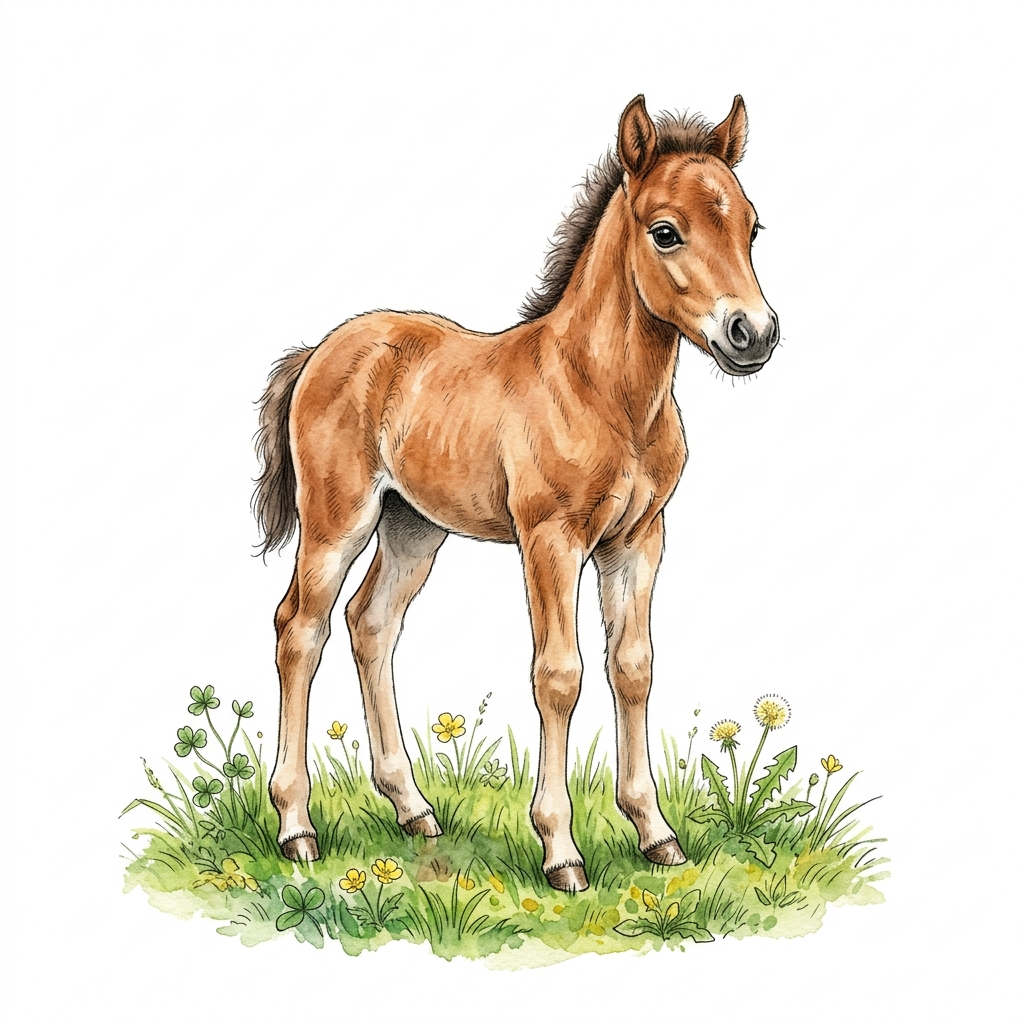
\includegraphics[width=0.85\linewidth]{vokab_300dpi/fellen.png} \\
            \vspace{0.3cm}
    }}
    \vspace{0.4em}
    \textbf{\Large D'Fëllen}\\
    \small\textit{(Le poulain / The foal)}
\end{minipage}
\end{noindent}
